\documentclass[aspectratio=169,xcolor={dvipsnames,table}]{beamer}
\usepackage[no-math,deluxe,haranoaji]{luatexja-preset}
\renewcommand{\kanjifamilydefault}{\gtdefault}
\renewcommand{\emph}[1]{{\upshape\bfseries #1}}
\usetheme{metropolis}
\metroset{block=fill}
\setbeamertemplate{navigation symbols}{}
\setbeamertemplate{blocks}[rounded][shadow=false]
\usecolortheme[rgb={0.7,0.2,0.2}]{structure}
%%%%%%%%%%%%%%%%%%%%%%%%%%
%% Change alert block colors
%%% 1- Block title (background and text)
\setbeamercolor{block title alerted}{fg=mDarkTeal, bg=mLightBrown!45!yellow!45}
\setbeamercolor{block title example}{fg=magenta!10!black, bg=mLightGreen!70}
%%% 2- Block body (background)
\setbeamercolor{block body alerted}{bg=mLightBrown!25}
\setbeamercolor{block body example}{bg=mLightGreen!15}
%%%%%%%%%%%%%%%%%%%%%%%%%%%
%%%%%%%%%%%%%%%%%%%%%%%%%%%
\usepackage{media9}
%%%%%%%%%%%%%%%%%%%%%%%%%%%
%% さまざまなアイコン
%%%%%%%%%%%%%%%%%%%%%%%%%%%
\usepackage{fontawesome}
\usepackage{figchild}
\usepackage{twemojis}
\usepackage{utfsym}
\usepackage{bclogo}
\usepackage{marvosym}
\usepackage{tipa}
%%%%%%%%%%%%%%%%%%%%%%%%%%%
\usepackage{tikz}
\usetikzlibrary{backgrounds}
\usepackage{tcolorbox}
\usepackage{tikzpeople}
\usepackage{xcolor}
\usepackage{amsmath}
\usepackage{manfnt}
%%%%%%%%%%%%%%%%%%%%%%%%%%%
%% 場合分け
\usepackage{cases}
%%%%%%%%%%%%%%%%%%%%%%%%%%%
% \myAnch{<名前>}{<色>}{<テキスト>}
% 指定のテキストを指定の色の四角枠で囲み, 指定の名前をもつTikZの
% ノードとして出力する. 図には remeber picture 属性を付けている
% ので外部から参照可能である.
\newcommand*{\myAnch}[3]{%
  \tikz[remember picture,baseline=(#1.base)]
    \node[draw,rectangle,#2] (#1) {\normalcolor #3};
}
%%%%%%%%%%%%%%%%%%%%%%%%%%%%
%% 音声リンク表示
\newcommand{\myaudio}[1]{\href{#1}{\faVolumeUp}}
%%%%%%%%%%%%%%%%%%%%%%%%%%%
% \myEmph コマンドの定義
%\newcommand{\myEmph}[3]{%
%    \textbf<#1>{\color<#1>{#2}{#3}}%
%}
\usepackage{xparse} % xparseパッケージの読み込み
\NewDocumentCommand{\myEmph}{O{} m m}{%
    \def\argOne{#1}%
    \ifx\argOne\empty
        \textbf{\color{#2}{#3}}% オプション引数が省略された場合
    \else
        \textbf<#1>{\color<#1>{#2}{#3}}% オプション引数が指定された場合
    \fi
}
%%%%%%%%%%%%%%%%%%%%%%%%%%%
\title{English is fun.}
\subtitle{The Cat and the Mice}
\author{}
\institute[]{}
\date[]

%%%%%%%%%%%%%%%%%%%%%%%%%%%%
%% TEXT
%%%%%%%%%%%%%%%%%%%%%%%%%%%%
\begin{document}
%%%%%%%%%%%%%%%%%%%%%%%%%%%%

%%%%%%%%%%%%%%%%%%%%%%%%%%%%%
\begin{frame}[plain]
  \titlepage
\end{frame}

\section*{授業の流れ}
\begin{frame}[plain]
  \frametitle{授業の流れ}
  \tableofcontents
\end{frame}
%%%%%%%%%%%%%%%%%%%%%%%%%%%%%%%%%%%%%%%%%%%
\section{単数と複数}
%%%%%%%%%%%%%%%%%%%%%%%%%%%%%%%%%%%%%%%%%%%
\begin{frame}[plain]\frametitle{ひとつとふたつ以上}
\begin{columns}
\begin{column}{.25\textwidth}
\IfFileExists{./images/one_book-crop.pdf}{%
\rotatebox{-90}{\includegraphics[width=1.1\textwidth]{./images/one_book-crop.pdf}
}}{naiyo}
\end{column}\pause
\begin{column}{.5\textwidth}\LARGE
a book
\end{column}
\end{columns}

\pause
\begin{columns}
\begin{column}{.25\textwidth}
\IfFileExists{./images/two_books-crop.pdf}{%
\rotatebox{-90}{\includegraphics[width=1.1\textwidth]{./images/two_books-crop.pdf}
}}{naiyo}
\end{column}\pause
\begin{column}{.5\textwidth}\LARGE
two book\myEmph[4]{Maroon}{s}
\end{column}

\end{columns}
\end{frame}
%%%%%%%%%%%%%%%%%%%%%%%%%%%%%%%%%%
\subsection{日本語と英語とのちがい}
%%%%%%%%%%%%%%%%%%%%%%%%%%%%%%%%%
\begin{frame}<1-15>[plain]\frametitle{日本語と英語のちがい}
\begin{columns}
\begin{column}[t]{.525\textwidth}
\begin{alertblock}{日本語}
\onslide<2->{わたしは1冊の本を持っています。}

\onslide<3->{わたしは2冊の本を持っています。}

\onslide<4->{わたしはたくさんの本を持っています。}

\onslide<5->{わたしは本を持っています。}
\end{alertblock}
\end{column}
\begin{column}[t]{.45\textwidth}
\begin{block}{英語}
\onslide<6->{I have \textcolor{NavyBlue}{\bfseries a book}.}%\,\,\,(I have \textcolor{NavyBlue}{\bfseries one book}.)

\onslide<7->{I have \textcolor{NavyBlue}{\bfseries two books}.}

\onslide<8->{I have \textcolor{NavyBlue}{\bfseries many books}.}

\onslide<9->{*I have \textcolor{Maroon}{\bfseries book}.}\onslide<10->{\,\,{}$\longleftarrow$これは\textcolor{Maroon}{だめ}}

\onslide<11->{I have \textcolor{NavyBlue}{\bfseries books}.}\onslide<12->{\,\,{}$\longleftarrow$これは\textcolor{NavyBlue}{\bfseries OK}}
\end{block}
\end{column}
\end{columns}

\begin{block}<13->{Topics for Today}\small
\begin{itemize}\setbeamertemplate{items}[square]
 \item<14->  {\textcolor{black}{単数形と複数形があります}}
 \item<15->  {\textcolor{black}{単数形を裸で使うことはできません\,\,\dbend}}\\
{複数形は裸で使えます}
\end{itemize}
      \end{block}
\end{frame}
%%%%%%%%%%%%%%%%%%%%%%%%%%%%
\section{複数形のつくり方}
%%%%%%%%%%%%%%%%%%%%%%%%%%%%%
\begin{frame}[plain]\frametitle{複数形のつくり方}
 
\Large
おしりに---sをつけます

a book $\longrightarrow$ book\textcolor{Maroon}{\bfseries s}

\end{frame}
%%%%%%%%%%%%%%%%%%%%%%%%%%%%%%%%%%%%%%
\begin{frame}[plain]\frametitle{Exercises 1}

\fcDog{0.4}{black}{1}\pause {\large a dog}\pause\,\, {\large (one dog)}\hspace{30pt}%
\pause
\fcDog{0.4}{black}{1}\fcDog{0.4}{black}{1}\pause {\large two dog\textcolor{Maroon}{\bfseries s}}
\pause

\bigskip

\fcCat{0.4}{black}{1}\pause {\large a cat}\hspace{50pt}%
\pause
\fcCat{0.4}{black}{1}\fcCat{0.4}{black}{1}\fcCat{0.4}{black}{1} \pause {\large three cat\textcolor{Maroon}{\bfseries s}}
\pause

\bigskip

\fcBirdB{0.4}{black}{1}\pause {\large a bird}\hspace{55pt}%
\pause
\fcBirdB{0.4}{black}{1}
\fcBirdB{0.4}{black}{1}
\fcBirdB{0.4}{black}{1}
\fcBirdB{0.4}{black}{1} \pause {\large four bird\textcolor{Maroon}{\bfseries s}}

\hfill{\tiny 0315}\,{\scriptsize \myaudio{./audio/005_singular_plural_01.mp3}}
\end{frame}
%%%%%%%%%%%%%%%%%%%%%%%%%%%%%%%%%%%%%%%%%%%%%%%%%%
\begin{frame}[plain]\frametitle{Exercises 2}

\fcBookB{0.4}{black}{1}\pause {\large a book}\hspace{20pt}%
\pause
\fcBookB{0.4}{black}{1}\fcBookB{0.4}{black}{1}%
\fcBookB{0.4}{black}{1}\fcBookB{0.4}{black}{1}%
\fcBookB{0.4}{black}{1} \pause%
\hfill{\large five book\textcolor{Maroon}{\bfseries s}}
\pause

\bigskip

\scalebox{.17}{\fcKey{0.4}{black}{2}}\,\,{}\pause {\large a key}\hspace{40pt}%
\pause
\scalebox{.17}{\fcKey{0.4}{black}{2}} \scalebox{.17}{\fcKey{0.4}{black}{2}} \scalebox{.17}{\fcKey{0.4}{black}{2}} \scalebox{.17}{\fcKey{0.4}{black}{2}} \scalebox{.17}{\fcKey{0.4}{black}{2}}\,\,\,\,\,\,\,\,\scalebox{.17}{\fcKey{0.4}{black}{2}}
\pause
\hfill{\large six key\textcolor{Maroon}{\bfseries s}}
\pause

\scalebox{.25}{\fcChairA{0.4}{black}{2}}\pause {\large a chair}\hspace{40pt}%
\pause
\scalebox{.25}{\fcChairA{0.4}{black}{2} \fcChairA{0.4}{black}{2} \fcChairA{0.4}{black}{2} \fcChairA{0.4}{black}{2} \fcChairA{0.4}{black}{2} \hspace{20pt}\fcChairA{0.4}{black}{2} \fcChairA{0.4}{black}{2}}
\pause
 \hfill{\large seven chair\textcolor{Maroon}{\bfseries s}}
\pause

\scalebox{1}{\fcBike{0.4}{black}{1}}\pause {\large a bike}\hspace{30pt}%
\pause
\scalebox{1}{\begin{tabular}{@{}lllll}
\fcBike{0.4}{black}{1}& \fcBike{0.4}{black}{1}& \fcBike{0.4}{black}{1}& \fcBike{0.4}{black}{1}& \fcBike{0.4}{black}{1}\\
 \fcBike{0.4}{black}{1}& \fcBike{0.4}{black}{1}& \fcBike{0.4}{black}{1}
	     \end{tabular}}
\pause

\vspace*{-25pt}
\mbox{}\hfill{\large eight bike\textcolor{Maroon}{\bfseries s}}

{\tiny 0413}\,{\scriptsize \myaudio{./audio/005_singular_plural_02.mp3}}
\end{frame}
%%%%%%%%%%%%%%%%%%%%%%%%%%%%%%%%%%%%%%%%%%%%%
\begin{frame}[plain]\frametitle{Exercises 3}

\usymW{2710}{1cm}\pause {\large a pencil}\hspace{20pt}%
\pause
\usymW{2710}{1cm}\usymW{2710}{1cm}\usymW{2710}{1cm}\usymW{2710}{1cm}\usymW{2710}{1cm}\hspace{15pt}
\usymW{2710}{1cm}\usymW{2710}{1cm}\usymW{2710}{1cm}\usymW{2710}{1cm}\pause

\mbox{}\hfill{\large nine pencil\textcolor{Maroon}{\bfseries s}}
\pause

\bigskip

\bigskip


\bcfleur\,\,\,\,\pause {\large a flower}\hspace{45pt}%
\pause
\bcfleur\bcfleur\bcfleur\bcfleur\bcfleur\hspace{15pt}
\bcfleur\bcfleur\bcfleur\bcfleur\bcfleur\hspace{10pt}
\pause
\hfill{\large ten flower\textcolor{Maroon}{\bfseries s}}

\hfill{\tiny 0224}\,{\scriptsize \myaudio{./audio/005_singular_plural_03.mp3}}

\pause
\begin{block}{Topics for Today}\small
 \begin{itemize}\setbeamertemplate{items}[square]
  \item 単数形と複数形があります
  \item 複数形は、最後に---sをつけます
  \item 単数形は裸では使えません\,\,\dbend\\
(複数形は裸でも使えます)
 \end{itemize}
     \end{block}
\end{frame}
%%%%%%%%%%%%%%%%%%%%%%%
\section{複数形のsの発音}
\begin{frame}[plain]\frametitle{複数形のsはどう発音するの}

\begin{enumerate}
 \item a dog~~~/~~~two dogs%
\hfill\makebox[40pt][l]{\onslide<12->{\textipa{/\textcolor<13->{Maroon}{g}/}$+$}\onslide<2->{\textipa{/z/}}}\hspace{180pt}\mbox{}
 \item a cat~~~/~~~three cats%
\hfill\makebox[40pt][l]{\onslide<12->{\textipa{/t/}$+$}\onslide<3->{\textipa{/s/}}}\hspace{180pt}\mbox{}
 \item a bird~~~~/~~~four birds%
\hfill\makebox[40pt][l]{\onslide<12->{\textipa{/\textcolor<13->{Maroon}{d}/}$+$}\onslide<4->{\textipa{/z/}}}\hspace{180pt}\mbox{}

 \item a book~~~/~~~five books%
\hfill\makebox[40pt][l]{\onslide<12->{\textipa{/k/}$+$}\onslide<5->{\textipa{/s/}}}\hspace{180pt}\mbox{}
 \item a key~~~/~~~six keys%
\hfill\makebox[40pt][l]{\onslide<12->{\textipa{/\textcolor<13->{Maroon}{i:}/}$+$}\onslide<6->{\textipa{/z/}}}\hspace{180pt}\mbox{}

 \item a chair~~~/~~~seven chairs%
\hfill\makebox[40pt][l]{\onslide<12->{\textipa{/\textcolor<13->{Maroon}{e\textrhookschwa}/}$+$}\onslide<7->{\textipa{/z/}}}\hspace{180pt}\mbox{}

 \item a bike~~~/~~~eight bikes%
\hfill\makebox[40pt][l]{\onslide<12->{\textipa{/k/}$+$}\onslide<8->{\textipa{/s/}}}\hspace{180pt}\mbox{}

 \item a pencil~~~~/~~~nine pencils%
\hfill\makebox[40pt][l]{\onslide<12->{\textipa{/\textcolor<13->{Maroon}{l}/}$+$}\onslide<9->{\textipa{/z/}}}\hspace{180pt}\mbox{}
 \item a flower~~~/~~~ten flowers%
\hfill\makebox[40pt][l]{\onslide<12->{\textipa{/\textcolor<13->{Maroon}{aU\textrhookschwa}/}$+$}\onslide<10->{\textipa{/z/}}}\hspace{180pt}\mbox{}
\end{enumerate}

\vspace{-20pt}

\hfill{\tiny 0525}\,{\scriptsize \myaudio{./audio/005_singular_plural_04.mp3}}

\begin{block}<11->{複数形のsの発音}\small
\onslide<11->{単語の最後の音に注目しよう}
\onslide<13->{$\longrightarrow$
有声音なら\textipa{/z/}\hspace{5pt} 無声音なら\textipa{/s/}}\,\dbend
\end{block}

\end{frame}
%%%%%%%%%%%%%%%%%
\begin{frame}[plain]{Exercises}
つぎの名詞を複数形にしてください。さらに語尾の発音が有声音の\textipa{/z/}になるか無声音の\textipa{/s/}になるか判断してください 

{\Large
\begin{enumerate}
 \item banana\visible<2->{\textcolor{Maroon}{s}}\hspace{10pt}\visible<3->{\textipa{/z/}}
 \item egg\visible<2->{\textcolor{Maroon}{s}}\hspace{10pt}\visible<4->{\textipa{/z/}}
 \item park\visible<2->{\textcolor{Maroon}{s}}\hspace{10pt}\visible<5->{\textipa{/s/}}
 \item lemon\visible<2->{\textcolor{Maroon}{s}}\hspace{10pt}\visible<6->{\textipa{/z/}}
 \item cup\visible<2->{\textcolor{Maroon}{s}}\hspace{10pt}\visible<7->{\textipa{/s/}}
 \item car\visible<2->{\textcolor{Maroon}{s}}\hspace{10pt}\visible<8->{\textipa{/z/}}
\end{enumerate}}

\hfill{\tiny 0339}\,{\scriptsize \myaudio{./audio/005_singular_plural_04b.mp3}}

\end{frame}
%%%%%%%%%%%%%%%%%
\begin{frame}[plain]{そういえば三単現のsはどう発音するの}
\Large
 \begin{enumerate}
  \item<1-> He swim\textbf<2->{\textcolor<2->{Maroon}{s}} in the river. \hfill\makebox[80pt][l]{\onslide<6->{\textipa{/m/} $+$} \onslide<2->{\textipa{/z/}}}\hspace{110pt}\mbox{}
  \item<1-> She live\textbf<3->{\textcolor<3->{Maroon}{s}} in Boston. \hfill\makebox[80pt][l]{\onslide<7->{\textipa{/v/} $+$} \onslide<3->{\textipa{/z/}}}\hspace{110pt}\mbox{}
  \item<1-> He drink\textbf<4->{\textcolor<4->{NavyBlue}{s}} coffee. \hfill\makebox[80pt][l]{\onslide<8->{\textipa{/k/} $+$} \onslide<4->{\textipa{/s/}}}\hspace{110pt}\mbox{}
  \item<1-> She write\textbf<5->{\textcolor<5->{NavyBlue}{s}} a book. \hfill\makebox[80pt][l]{\onslide<9->{\textipa{/t/} $+$} \onslide<5->{\textipa{/s/}}}\hspace{110pt}\mbox{}

 \end{enumerate}

\normalsize
\begin{block}<10->{Topics for Today}
\begin{description}[三単現のsの発音]
 \item[三単現のsの発音] 
動詞の最後の音が有声音なら\textipa{/z/}\\
\phantom{動詞の最後の音が}無声音なら\textipa{/s/}\,\dbend\\
\mbox{}
\end{description}
\end{block}
{\tiny 0139}\,{\scriptsize \myaudio{./audio/005_singular_plural_a.mp3}}\hfill\onslide<11->{{\scriptsize 複数形のsの発音と同じかんがえかたです}}
\end{frame}

%%%%%%%%%%%%%%%%%%%%%%%%%%%%%%%%%%%%%%%%%%%%%
\section{注意すべき複数形1 --- yで終わる名詞の複数形}
%%%%%%%%%%%%%%%%%%%%%%%%%%%%%%%%%%%%%%%%%%%%%%
\begin{frame}[plain]{yで終わる名詞の複数形}\Large
\begin{enumerate}
 \item<1-> a b\textbf<14->{\textcolor<14->{YellowOrange}{o}}y $\rightarrow$ \visible<2->{boy\textcolor{Maroon}{\bfseries s}}
 \item<3-> a d\textbf<14->{\textcolor<14->{YellowOrange}{a}}y $\rightarrow$ \visible<4->{day\textcolor{Maroon}{\bfseries s}}
 \item<5-> a t\textbf<14->{\textcolor<14->{YellowOrange}{o}}y $\rightarrow$ \visible<6->{toy\textcolor{Maroon}{\bfseries s}}
 \item<7-> a ci\textbf<14->{\textcolor<14->{CarnationPink}{t}}y $\rightarrow$ \visible<8->{cit\textcolor{NavyBlue}{\bfseries ies} (*citys)}
 \item<9-> a count\textbf<14->{\textcolor<14->{CarnationPink}{r}}y $\rightarrow$ \visible<10->{countr\textcolor{NavyBlue}{\bfseries ies} (*countrys)}
 \item<11-> a ba\textbf<14->{\textcolor<14->{CarnationPink}{b}}y $\rightarrow$ \visible<12->{bab\textcolor{NavyBlue}{\bfseries ies} (*babys)}
\end{enumerate} 

\normalsize
\begin{block}<13->{Topics for Today}
\onslide<13->{yの直前の文字に注目しよう}
\onslide<15->{$\longrightarrow$
\begin{tabular}[t]{ll}
 母音字なら&原則どおり(sをつけるだけ) \\
 子音字なら&yをiに変えてes 
\end{tabular}
\dbend}\\
{\tiny 0211}\,{\scriptsize \myaudio{./audio/005_singular_plural_b.mp3}}\hfill\onslide<15->{\scriptsize 母音字: aeiou\hspace{10pt}子音字: それ以外}
\end{block}

\end{frame}
%%%%%%%%%%%%%%%%%
\begin{frame}[plain]{Exercises}

例にならって、複数形にしてください(例:book $\longrightarrow$ books)

 \Large

\begin{enumerate}
 \item<1-> key \onslide<2->{$\longrightarrow$ keys}\hfill{}{\scriptsize key \textipa{/k\'\i:/} 鍵}
 \item<1-> monkey \onslide<3->{$\longrightarrow$ monkeys}\hfill{}{\scriptsize monkey \textipa{/m\'\textturnv Nki/} サル}
 \item<1-> body \onslide<4->{$\longrightarrow$ bodies}\hfill{}{\scriptsize body \textipa{/b\'Adi/} 身体}
 \item<1-> story \onslide<5->{$\longrightarrow$ stories}\hfill{}{\scriptsize story \textipa{/st\'O:ri/} 物語}
 \item<1-> family \onslide<6->{$\longrightarrow$  families}\hfill{}{\scriptsize family \textipa{/f\'\ae m\textschwa li/} 家族}
\end{enumerate}

\hfill{\tiny 0151}\,{\scriptsize \myaudio{./audio/005_singular_plural_c.mp3}}
\end{frame}
%%%%%%%%%%%%%%%%%%
\begin{frame}[plain]{そういえばyで終わる動詞の三単現は?}

yで終わる動詞の三単現

\Large
 \begin{enumerate}
  \item<1-> \begin{enumerate}
	     \item<1-> They drink tea. 
	     \item<2-> Helen \onslide<3->{drink\textbf{\textcolor{Maroon}{s}} tea.}
	    \end{enumerate}
  \item<1-> \begin{enumerate}
	 \item<1-> They play the piano.
	 \item<4-> He \onslide<5->{play\textbf{\textcolor{Maroon}{s}} the piano.}
	\end{enumerate}
  \item<1-> \begin{enumerate}
	 \item<1-> They study English.
	 \item<6-> She \onslide<7->{stud\textbf{\textcolor{NavyBlue}{ies}}  English. \hspace{10pt}(*studys)}
	\end{enumerate}
 \end{enumerate}
 
\normalsize
\begin{block}<8->{Topics for Today}\small
\begin{description}[yで終わる動詞の三単現のつくり方]
 \item[yで終わる動詞の三単現のつくり方] 
yの直前が母音字ならs(原則どおり)\\
\phantom{yの直前が}子音字ならyをiに変えてes\hfill\dbend\\
\mbox{}\hfill{\scriptsize 母音字: aeiou\hspace{10pt}子音字: それ以外   }
\end{description}
\end{block}
\hfill\onslide<9->{{\scriptsize yで終わる名詞の複数形のつくり方と同じです}}


\end{frame}
%%%%%%%%%%%%%%%%%
\begin{frame}[plain]{Exercises}
 
つぎの動詞を三単現にしてください

\Large
\begin{enumerate}
 \item buy\,\,\,\,{\small \textipa{/b\'aI/}(買う)}\hfill\visible<2->{buys}\hspace{200pt}\mbox{}
 \item enjoy\,\,\,\,{\small \textipa{/IndZ\'OI/}(楽しむ)}\hfill\visible<3->{enjoys}\hspace{200pt}\mbox{}
 \item say\,\,\,\,{\small \textipa{/s\'eI/}(言う)}\hfill\visible<4->{says}\,\,\,\visible<9->{\textipa{/s\'ez/}}\hspace{160pt}\mbox{}
 \item cry\,\,\,\,{\small \textipa{/kr\'aI/}(泣く)}\hfill\visible<5->{cries}\hspace{200pt}\mbox{}
 \item carry\,\,\,\,{\small \textipa{/k\'\ae ri/}(運ぶ)}\hfill\visible<6->{carries}\hspace{200pt}\mbox{}
 \item fly\,\,\,\,{\small \textipa{/fl\'aI/}(飛ぶ)}\hfill\visible<7->{flies}\hspace{200pt}\mbox{}
% \item hurry\hspace{40pt}\visible<2->{hurries}
 \item try\,\,\,\,{\small \textipa{/tr\'aI/}(試す)}\hfill\visible<8->{tries}\hspace{200pt}\mbox{}
% \item worry\hspace{40pt}\visible<2->{worries}
\end{enumerate}

\hfill{\tiny 0408}\,{\scriptsize \myaudio{./audio/005_singular_plural_d.mp3}}


\end{frame}
%%%%%%%%%%%%%%%%
\section{注意すべき複数形2 --- esをつける複数形}
\begin{frame}[plain]{注意すべき複数形}

\scalebox{.5}{\fcBus{0.4}{black}{2}}\hspace{15pt}\pause {\LARGE a bus}\hspace{15pt}{\Large \textipa{/b\'2s/}}
\pause

\bigskip

\bigskip

\scalebox{.5}{\fcBus{0.4}{black}{2}\hspace{15pt}\fcBus{0.4}{black}{2}}\hspace{15pt}
\pause {\LARGE two  bus\textcolor{orange}{\bfseries es}}\hspace{15pt}{\Large \textipa{/iz/}}\hfill{}(*buss)

{\tiny 0057}\,{\scriptsize \myaudio{./audio/005_singular_plural_05.mp3}}
\end{frame}
%%%%%%%%%%%%%%%%%%%%%%%%%%%%%%%%%%%%%%%%%%%%%%%%%%%%%%
\begin{frame}[plain]{注意すべき複数形}
\scalebox{.4}{\fcPotato{0.4}{black}{2}}\hspace{15pt}
\pause
{\LARGE a potato}\hspace{15pt}{\Large \textipa{/p@t\'eItoU/}} 
\pause

\bigskip

\bigskip

\scalebox{.4}{\fcPotato{0.4}{black}{2}\fcPotato{0.4}{black}{2}\fcPotato{0.4}{black}{2}}\hspace{15pt}
\pause
{\LARGE three  potato\textcolor{orange}{\bfseries es}}\hspace{10pt}{\Large \textipa{/z/}}

{\tiny 0059}\,{\scriptsize \myaudio{./audio/005_singular_plural_06.mp3}}
\end{frame}
%%%%%%%%%%%%%%%%%%%%%%%%%%%%%%%%%%%%%%%%
\begin{frame}[plain]\frametitle{注意すべき複数形}

{\Large `s'ではなく\textcolor{orange}{`es'}をつける複数形があります}
\pause

\bigskip

\begin{block}{--- $\rightarrow$ ---es}
a bus \pause$\longrightarrow$ bus\textcolor{orange}{es}\pause%
\hfill\makebox[20pt]{\textipa{/iz/}}\hspace*{250pt}\pause

a class \pause$\longrightarrow$ class\textcolor{orange}{es}\pause
\hfill\makebox[20pt]{\textipa{/iz/}}\hspace*{250pt}\pause

a box \pause $\longrightarrow$ box\textcolor{orange}{es}\pause
\hfill\makebox[20pt]{\textipa{/iz/}}\hspace*{250pt}\pause

a potato \pause$\longrightarrow$ potato\textcolor{orange}{es}\pause
\hfill\makebox[20pt]{\textipa{/z/}}\hspace*{250pt}\pause

a tomato \pause$\longrightarrow$ tomato\textcolor{orange}{es}\pause
\hfill\makebox[20pt]{\textipa{/z/}}\hspace*{250pt}
\end{block}
\end{frame}
%%%%%%%%%%%%%%%%%%%%%%%%%%%%%%%%%%%%%%%%%%%%%%%%%%
\begin{frame}[plain]\frametitle{Pronunciation}

\begin{enumerate}
 \item a bus~~~\pause{}/~~~buses\pause%
\hfill\makebox[40pt][l]{\onslide<11->{\textipa{/b\'2s/} $+$ \textipa{/Iz/}}}\hspace{180pt}\mbox{} \item a class~~~~\pause{}/~~~classes\pause%
\hfill\makebox[40pt][l]{\onslide<12->{\textipa{/kl\'\ae s/} $+$ \textipa{/Iz/}}}\hspace{180pt}\mbox{}
 \item a box~~~\pause{}/~~~boxes\pause%
\hfill\makebox[40pt][l]{\onslide<13->{\textipa{/b\'Aks/} $+$ \textipa{/Iz/}}}\hspace{180pt}\mbox{}
 \item a potato~~~\pause{}/~~~potatoes\pause%
\hfill\makebox[40pt][l]{\onslide<14->{\textipa{/p@t\'eItoU/} $+$ \textipa{/z/}}}\hspace{180pt}\mbox{} \item a tomato~~~\pause{}/~~~tomatoes%
\hfill\makebox[40pt][l]{\onslide<15->{\textipa{/t@m\'eItoU/} $+$ \textipa{/z/}}}\hspace{180pt}\mbox{}
 \end{enumerate}

\bigskip

\bigskip

\mbox{}\hfill{\tiny 0309}\,{\scriptsize \myaudio{./audio/005_singular_plural_07.mp3}}
\end{frame}
%%%%%%%%%%%%%%%%%%%%%%%%%%%%%%%%%%%%%%%%%%%%%%%%%%%
\section{不規則な複数形}
\begin{frame}[plain]{注意すべき複数形}
\scalebox{5}{\ManFace}\hspace{15pt}
\pause
{\LARGE a man}\pause\hspace{15pt}{\Large \textipa{/m\'\ae n/}}
\pause

\bigskip

\bigskip

\scalebox{5}{\ManFace\hspace{5pt}\ManFace\hspace{5pt}\ManFace}\hspace{15pt}
\pause
{\LARGE three  \textcolor{orange}{\bfseries men}}\pause\hspace{15pt}{\Large \textipa{/m\'en/}}

\bigskip

\bigskip

\mbox{}\hfill{\tiny 0122}\,{\scriptsize \myaudio{./audio/005_singular_plural_08.mp3}}
\end{frame}
%%%%%%%%%%%%%%%%%%%%%%%%%%%%%%%%%%%%%%%%%%%%%%%%%%%%%%%
\begin{frame}[plain]{注意すべき複数形}
\scalebox{5}{\WomanFace}\pause\hspace{15pt} {\LARGE a woman}%
\pause\hspace{15pt}{\Large \textipa{/w\'Um\textschwa n/}}
\pause

\bigskip

\bigskip

\scalebox{5}{\WomanFace \WomanFace \WomanFace \WomanFace} \hspace{25pt}
\pause
{\LARGE four  \textcolor{orange}{\bfseries women}}%
\pause\hspace{15pt}{\Large \textipa{/w\'ImIn/}}

\bigskip

\bigskip

\mbox{}\hfill{\tiny 0057}\,{\scriptsize \myaudio{./audio/005_singular_plural_09.mp3}}
\end{frame}
%%%%%%%%%%%%%%%%%%%%%%%%%%%%%%%%%%
\begin{frame}[plain]{注意すべき複数形}
\scalebox{.7}{%
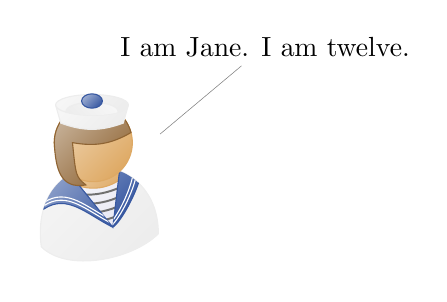
\begin{tikzpicture}
\node[sailor,female,minimum size=1.5cm,
anchor=south,pin={85:I am Jane. I am twelve.}] at (6.25cm,0) {};
%\node[charlie,minimum size=1.5cm,
%anchor=south,,pin={105:I am Bob.}] at (5cm,0) {};
\end{tikzpicture}
}\pause
\hspace{80pt}{\LARGE a child}%
\pause\hspace{15pt}{\Large \textipa{/tS\'aIld/}}
\pause

\bigskip

\scalebox{.7}{%
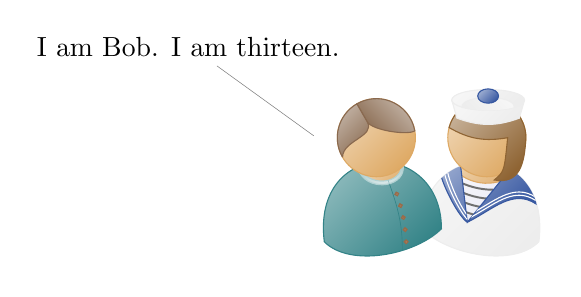
\begin{tikzpicture}
\node[sailor,female,mirrored,minimum size=1.5cm,
anchor=south] at (6.25cm,0) {};
\node[charlie,minimum size=1.5cm,
anchor=south,,pin={105:I am Bob. I am thirteen.}] at (5cm,0) {};
\end{tikzpicture}
}\pause
\hspace{45pt}{\LARGE two \textcolor{orange}{\bfseries children}}%
\pause\hspace{15pt}{\Large \textipa{/tS\'Ildr\textschwa n/}}


\bigskip

\bigskip

\mbox{}\hfill{\tiny 0058}\,{\scriptsize \myaudio{./audio/005_singular_plural_10.mp3}}
\end{frame}
%%%%%%%%%%%%%%%%%%%%%%%%%%%%%%%%%%%%%%%%%%
\begin{frame}[plain]{注意すべき複数形}
 \fcMouse{.4}{gray}{.5}\pause\hspace{190pt}{\LARGE a mouse}%
\pause\hspace{15pt}{\Large \textipa{/m\'aUs/}}


\bigskip

\bigskip

\fcMouse{.4}{gray}{.5}\fcMouse{.4}{gray}{.5}\fcMouse{.4}{gray}{.5}\fcMouse{.4}{gray}{.5}\pause\hspace{50pt}{\LARGE four \textcolor{BurntOrange}{\bfseries mice}}%
\pause\hspace{15pt}{\Large \textipa{/m\'aIs/}}


\bigskip

\bigskip

\mbox{}\hfill{\tiny 0058}\,{\scriptsize \myaudio{./audio/005_singular_plural_11.mp3}}
\end{frame}
%%%%%%%%%%%%%%%%%%%%%%%%%%%%%%%%%%%%%%%%%%
\begin{frame}[plain]\frametitle{Pronunciation}

\begin{enumerate}
 \item a man~~~\pause{}/~~~men\pause
 \item a woman~~~\pause{}/~~~women\pause
 \item a child~~~\pause{}/~~~children\pause
 \item a mouse~~~\pause{}/~~~mice
  \end{enumerate}
\pause

\bigskip

\bigskip

\mbox{}\hfill{\tiny 0232}\,{\scriptsize \myaudio{./audio/005_singular_plural_12.mp3}}
\end{frame}
%%%%%%%%%%%%%%%%%%%
\begin{frame}[plain]{まとめ1}
 \begin{block}{基本}\small
\begin{itemize}\setbeamertemplate{items}[square]
 \item  単数形と複数形があります\hfill{}a book / books
 \item 複数形は最後に---sをつけます(原則)
 \item  単数形を裸で使うことはできません\hfill{}*I have book.\,\,\dbend\\
複数形は裸で使えます\hfill{}I have books.\,\phantom{\dbend}\mbox{}
\end{itemize}
      \end{block}

\pause

\begin{block}{複数形のsの発音}\small
\begin{itemize}\setbeamertemplate{items}[square]
 \item 単語の最後の音が有声音なら\textipa{/z/}\,\,\dbend\hfill{}dogs \textipa{/d\'Agz/}
 \item \phantom{単語の最後の音が}無声音なら\textipa{/s/}\hfill{}books \textipa{/b\'Uks/}
\end{itemize}
\end{block}
\end{frame}
%%%%%%%%%%%%%%%%%%%%%%%
\begin{frame}[plain]{まとめ2}
 \begin{block}{yで終わる名詞の複数形}
\begin{itemize}\setbeamertemplate{items}[square]
 \item yの直前の文字が母音字なら、原則どおり(sをつけるだけ)\hspace{15pt}\dbend
 \item \phantom{yの直前の文字が}子音字なら、yをiに変えてes 
\end{itemize}
\hfill{\scriptsize 母音字: aeiou\hspace{10pt}子音字: それ以外}
\end{block}

\pause

\begin{columns}
\begin{column}{.45\textwidth}
\begin{block}{---esをつける複数形}
a bus $\longrightarrow$ bus\textcolor{orange}{es}%
\hfill\makebox[20pt]{\textipa{/iz/}}\hspace*{25pt}

a class $\longrightarrow$ class\textcolor{orange}{es}
\hfill\makebox[20pt]{\textipa{/iz/}}\hspace*{25pt}

a box  $\longrightarrow$ box\textcolor{orange}{es}
\hfill\makebox[20pt]{\textipa{/iz/}}\hspace*{25pt}

a potato $\longrightarrow$ potato\textcolor{orange}{es}
\hfill\makebox[20pt]{\textipa{/z/}}\hspace*{25pt}

a tomato $\longrightarrow$ tomato\textcolor{orange}{es}
\hfill\makebox[20pt]{\textipa{/z/}}\hspace*{25pt}
\end{block}
{\scriptsize ここまでは最後の1文字がsというのは共通}
\end{column}
\pause
\begin{column}{.45\textwidth}
\begin{block}{不規則な複数形}
 \begin{enumerate}
 \item a man~~~\rightarrow{}~~~men
 \item a woman~~~\rightarrow{}~~~women
 \item a child~~~\rightarrow{}~~~children
 \item a mouse~~~\rightarrow{}~~~mice
  \end{enumerate}
\end{block}
\end{column}
\end{columns}
\end{frame}
\end{document}
